

\chapter{Análisis de Opiniones}

	Para definir el concepto de Análisis de Opiniones es necesaria una breve introducción al Procesamiento del Lenguaje Natural.

\section{Procesamiento del Lenguaje Natural} \label{conceptsentiment}	
	
	 El Procesamiento del Lenguaje Natural (PLN) es un campo de la Inteligencia Artificial que se encarga de estudiar la comunicación que surge entre personas y máquinas. El objeto de estudio del PLN es, por tanto, el lenguaje. Para que las máquinas puedan conseguir capacidad de procesamiento y de generación del lenguaje, es necesario que se tenga comprensión total de la lengua. De esta misión se encarga la Lingüística, que trata de caracterizar y explicar los procedimientos del lenguaje.
	
	El procedimiento usual de un sistema PLN se divide en tres fases principales: análisis sintáctico, semántico y pragmático. En la práctica, estas fases no son suficientes. Esto se debe a que no es viable realizar el análisis sintáctico de un texto sin haber identificado las palabras y las oraciones además de la información morfológica de las palabras que componen la frase. Así, a las tres fases anteriores habría que añadir dos nuevas fases: \textit{tokenización} y análisis léxico.
	
	
	A continuación observamos el flujo de trabajo que seguiría un sistema PLN. La funcionalidad de la cada una de las fases sería:

		\begin{minipage}{.65\textwidth}
			\begin{enumerate}% never number things manually!
				\item \textit{Tokenización: }  Identificar las unidades en las que se divide el mensaje, \textit{tokens}.
				\item Análisis léxico: Obtiene información de los \textit{tokens} a partir de la función que desempeñan en la oración.
				\item Análisis sintáctico: Obtiene las relaciones y dependencias existentes entre los elementos que componen la oración.
				\item Análisis Semántico: Obtención de la intención del autor a partir de la información obtenida en la fase anterior. Busca descubrir el significado de la frase.
				\item Análisis Pragmático: Busca las conexiones entre oraciones para dar un sentido global al discurso.
			\end{enumerate}
		\end{minipage}
		\begin{minipage}{.35\textwidth}
			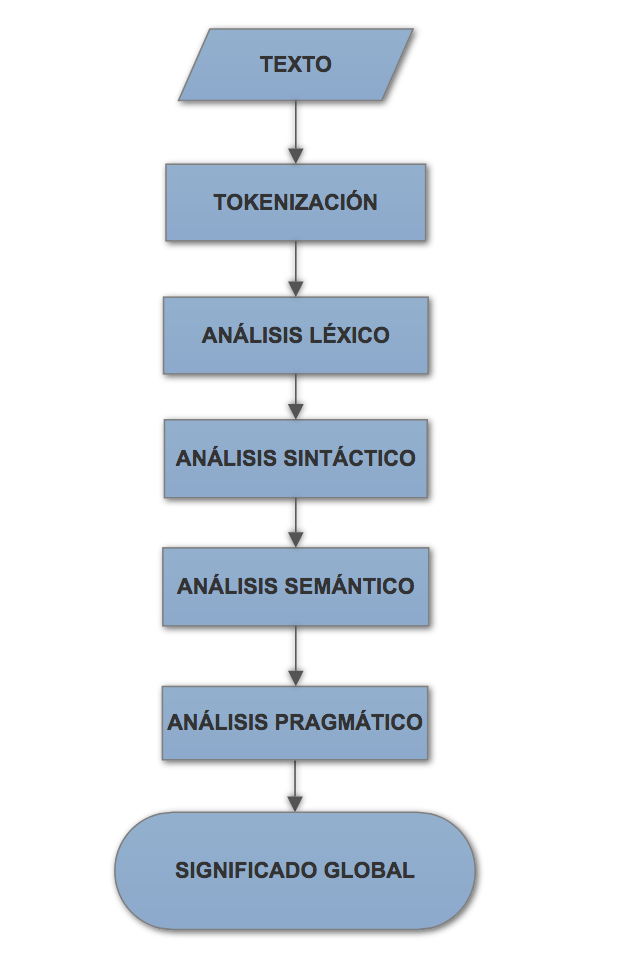
\includegraphics[width=1\linewidth]{imagenes/flujo}
		\end{minipage}
		
	La búsqueda del entendimiento del lenguaje no es la única misión del PLN. También persigue la generación automática de lenguaje, aunque no va a ser en lo que centremos esta memoria.
	
	
	
\section{Concepto de Análisis de opiniones}\label{conceptoSA}

	El Análisis de opiniones (AO) recibe muchos nombres dado a la evolución histórica que ha tenido: Análisis de Sentimientos, Minería de Opiniones, etc. A partir de ahora y durante todo el proyecto nos referiremos a él como Análisis de Opiniones.
	
	Definimos el Análisis de Opiniones como el estudio computacional de opiniones, sentimientos y emociones expresadas en un texto. Puede ser considerado como un proceso de clasificación cuyo fin es decidir la polaridad del sentimiento expresada en el texto. La dificultad de esta ciencia recaerá en el objeto de estudio pues se trata de información desestructurada, teniendo que convertirlos en datos estructurados. 
	
	\subsection{Concepto de Opinión}\label{opinion}
	
		Como hemos comentado en la sección anterior, el objetivo del AS consite en la extracción de información a partir de textos. Fundamental para definir ese concepto será la definición de su objeto de estudio, el concepto de opinión.
		
		Una primera aproximación para la definición de opinión la encontramos en el diccionario de la RAE, una opinión es un ``juicio o valoración que se forma una persona respecto de algo o de alguien.'' De esta definición podemos destacar varias cosas. Claramente una opinión es subjetiva, juicio o valor, pero también vemos que se hace énfasis en  quién crea la opinión y sobre qué. Empezamos así a vislumbrar que la opinión estará formada por varios elementos. 
		
		Para hacer más énfasis en este concepto de opinión formada por varios elementos, veamos un ejemplo concreto:
		
			\begin{center}
			\begin{minipage}{0.9\linewidth}
				\vspace{5pt}%margen superior de minipage
				{\small
					\textit{[1] El pasado jueves fui con un grupo de amigos a cenar a un restaurante. [2] Pedí unos macarrones a la carbonara que estaban deliciosos. [3] Sin embargo, el postre no me gustó nada, pedí una tarta de queso. [4] Creo que en este sentido acertó más mi amiga María que pidió la tarta de tres chocolates, ¡le encantó! [5] En cuanto al precio, no estaba nada mal para la cantidad que servían. [6] También hay que  tener en cuenta que se encontraba a las afueras, solo se puede acceder en coche.}
				}
				\vspace{5pt}%margen inferior de la minipage
			\end{minipage}
		\end{center}
	

	Si observamos el texto anterior con la intención de extraer una opinión global sobre el restaurante, encontramos que se da información ``contradictoria'' pues hay oraciones que expresan opiniones negativas, positivas e incluso neutras. La oración [1] expresa un hecho, sin ningún juicio de valor. Por su parte, las oraciones [2], [4] y[5] expresan sentimiento positivo mientras que las oraciones [3] y [6] expresan alguna opinión negativa. Vemos que cada una de estos juicios se realizan a ciertos elementos del restaurante, por lo que será algo a tener en cuenta dependiendo de si queremos determinar opinión de la entidad (restaurante) o de cada uno de sus componentes. Otro detalle presente en el ejemplo es que no siempre la persona que juzga algo es el autor del texto. En este caso, en la frase [4] el autor expresa que a su amiga le encantó su postre. Destacar también la importancia del tiempo a la hora de realizar un juicio de valor pues nuesta opinión puede variar a lo largo del tiempo. 
	
	En este punto, podemos considerar la opinión como una cuádrupla \textit{(o, p, h, t)} donde \textit{o} representa el objeto sobre el que recae la opinión, \textit{p} la polaridad de la misma, \textit{h} el autor y \textit{t} el tiempo en el que se produjo.
	
	Si nos fijamos en la frase [3] que expresa un sentimiento negativo, vemos que la opinión negativa no es sobre el restaurante en su conjunto si no que  es hacia un postre concreto. Según la definición de opinión como una cuádrupla \textit{(o, p, h, t)} su polaridad recaería sobre el objeto en cuestión, el restaurante. Así, surge la necesidad de considerar que el objeto pueda ser dividido en diferentes componentes. Definimos como entidad \textit{e} a un producto, servicio, tema, persona, organización o ente. Esta entidad se representa mediante \textit{(T,W)} donde \textit{T} es una jerarquía de componentes y \textit{W} el conjunto de atributos de \textit{e}. 
	
	Con esta nueva consideración llegamos a nuestra definición de opinión, introducida en \cite{liu}. Una opinión estaría formada por una quíntupla $(e_i, a_{ij}, p_{ijkl}, h_{k}, t_{l})$ donde $e_i$ representa la entidad, $a_ij$ sería el atributo de $e_i$ sobre el que recae la opinión, $p_{ijkl}$ se correspondería con la polaridad de la opinión que se hace sobre el aspecto $a_{ij}$ en el momento de tiempo $t_{l}$ por la persona $h_{k}$ y, por último, $h_{k}$ y $t_{l}$ la persona y el tiempo en que se realiza el juicio de valor respectivamente.
		 
		
	\subsection{Niveles de clasificación}\label{nivelesSA}
	
	%Aqui hacer mucho énfasis en lo importante que es hacerlo por entidades -> Dar importancia a mi trabajo
	
	Como ya hemos introducido, el objetivo final del Análisis de Opiniones es la clasificación de un texto según su polaridad. Ahora bien, a la hora de clasificar la polaridad de un texto podemos considerar tres niveles:
	
	\begin{enumerate}
		\item \textbf{Nivel de texto: } Analiza el documento completo y asigna una polaridad global al documento en su conjunto. Es el nivel más general y, por tanto, menos preciso.
		\item \textbf{Nivel de sentencias: } Detecta el sentimiento en frases. Está muy relacionado con la subjetividad ya que esta se expresa en frases y no en documentos largos. Obtendríamos uan clasificación más precisa del sentimiento.
		\item \textbf{Nivel de aspectos o entidades: } Detecta el sentimiento u opinión y la entidad a la que se refiere. Es el nivel más preciso de análisis, pues no produce generalizaciones si no que se identifica una polaridad con un aspecto concreto.
	\end{enumerate}
	
	 Como ya hemos comentado, nuestro proyecto se centrará en el último de estos niveles de clasificación. La importancia de esta especificación queda reflejada en el ejemplo que pusimos en la sección \ref{opinion}. Además, una vez tengamos clasificada la polaridad de los diferentes aspectos o entidades, es fácilmente extrapolable al resto de niveles de clasificación. Podemos obtener la clasificación a nivel de sentencias simplemente con la combinación de la polaridad de cada uno de los aspectos que aparecen en la sentencia y análogamente con la clasificación a nivel de texto.